

\documentclass{article} 

\usepackage{amsmath} % \usepackage is a command that allows you to add functionality to your LaTeX code
\usepackage{graphicx}
\usepackage{hyperref}

\graphicspath{ {./plots} }

\title{Raport for Flight Delay Predicion Project} % Sets article title
\author{Dominik Olejarz, Patryk Rybak, Maksymilian Wnuk} % Sets authors name
\date{\today} % Sets date for date compiled

% The preamble ends with the command \begin{document}
\begin{document} % All begin commands must be paired with an end command somewhere
 \maketitle
    
 \section{Problem Statement} % creates a section

Our goal is to predict flight delays and, in the future, expand the program to calculate the most probable delay values. Throughout our work, we will utilize a dataset containing flight information from 2017 to 2018, provided by the Bureau of Transportation Statistics in conjunction with the Weather API. The primary focus is to examine the correlation between weather conditions and flight delays.

Our approach centers around machine learning techniques, and we will employ statistical learning models using Python. The aim is to forecast flight delays and in future provide precise values of delays. We believe that our project can contribute to improving the travel experience by offering more accurate information about potential flight delays.

    
 \section{Data downloading}
Getting data for our machine learning models requires two combined datasets, 
flights and weather:
	\subsection{Flights data}
		We are getting 2017-2018 flights data from this: \url{https://www.kaggle.com/datasets/yuanyuwendymu/airline-delay-and-cancellation-data-2009-2018} dataset from well known site Kaggle.
		It contains of columns:	
			\begin{itemize}
\item Airline - company name of airline operating flight
\item Origin city  - city of departure
\item Destination city - city of arrival
\item CRS dep time, CRS arr time - expected time of departure and arrive in (weirdly represented) unsigned integer in which 
		least signitficant digits represent minutes and most significant represent hours
\item Arr time - factual time of arrive
\item Cancelled, Delay - boolean values signifying whether the flight was cancelled or (respectively) delayed
\item Distance  - distance between origin and destination
\item Arrive delay - signed integer value of delay
				
			\end{itemize}

	\subsection{Weather data}
		Fetching data for weather requires more work than just downloading a csv file.
		We will be downloading it by making api requests to \url{https://www.visualcrossing.com}.
		Thanks to Visual Crossing\textsuperscript{\tiny\textregistered} company, we were able to make those requests in unlimited way.
		We contacted their support and then they gave us access to unlimited synchronous API queries. 	\\
		However, we couldn't make 12 millions of api queries. Here we encounter
		our first problem.\\
		\textbf{Solution:}\\
		It wasn't that easy, we came up with idea of sending one request for one year for certain place.
		Api allowed us to make such queries.  So in order to do this, we send request of getting timeline of whole year,
		given city, year (2017 and later 2018), state, starting and finishing date (1'st january to 31'st december). What we get is a whole 					timeline
		for the city. We can now easily merge data from flights with weathers, using matrix with weather for 
		according place and time.\\

		We get columns:

			\begin{itemize}
\item Temperature - in fahrenheit scale
\item Cloudcover - how much of the sky is covered in percentage
\item Monphase - fractional portion through moon lunation cycle, 0-new moon to 0.5 ful moon and back to 1.0 next new moon
\item Windspeed, windgust and winddir
\item Snow and snowdepth - amount of snow that fell and depth of snow on the ground
\item Dew - dew point temperature in fahrenheit
\item Humidity - percentage of relative humidity
\item Boolean represented variables:
	\begin{itemize}
		\item ice
		\item freezing rain
		\item snow
		\item rain
	\end{itemize}
				
			\end{itemize}
\section{Data preprocessing}

\subsection{NaN's removal}
Dataset contains of lots of NaN's. We removed all of them, by removing rows that contained them. Data loss
was incredibly low, we lost about 10,000 of rows that contained at least one NaN, which is great. Additionally,
we removed columns that contained A LOT of NaN's. Those columns were:
	\begin{itemize}
		\item Windgust -75.22\% NaNs
		\item Snow - 8.13\% NaNs
		\item Snowdepth - 8.13\% NaNs
		\item ID,id - 55\% and 44\% respectively,no idea why so many nans, its just id's whose we don't even use in our model.
	\end{itemize}

However, we are not sure if that was proper way of doing this, hence we ask ourselves: does snow affect flight delays? How about snowdepth and wingust? Later on we can always retrieve those columns and check correlation.

\subsection{Normalization}
In order to normalize data, we will be using StandardScaler() class from sklearn.preprocessing library.
It was vital to make our dataset have common scale in order to maybe speed up and (?)make models work better.

\subsection{Mapping strings to integers}
In machine learning we would like to represent strings as integers. We will do that, by mapping destination and origin cities to integers
as json file. This file is in \textit{Flight-Delay-Prediction/ml} folder, named mappings.json. Additionally, we will map some weather data. Under column conditions there are many string representations, but we will represent it as integers (also in file mappings.json).

\newpage
\section{Explanatory Data Analysis (EDA) plots}
In this section we will look at plots describing data in our dataset.\\
Those plots are constructed in python' file \textit{EDA\_plottings.py} 
	
	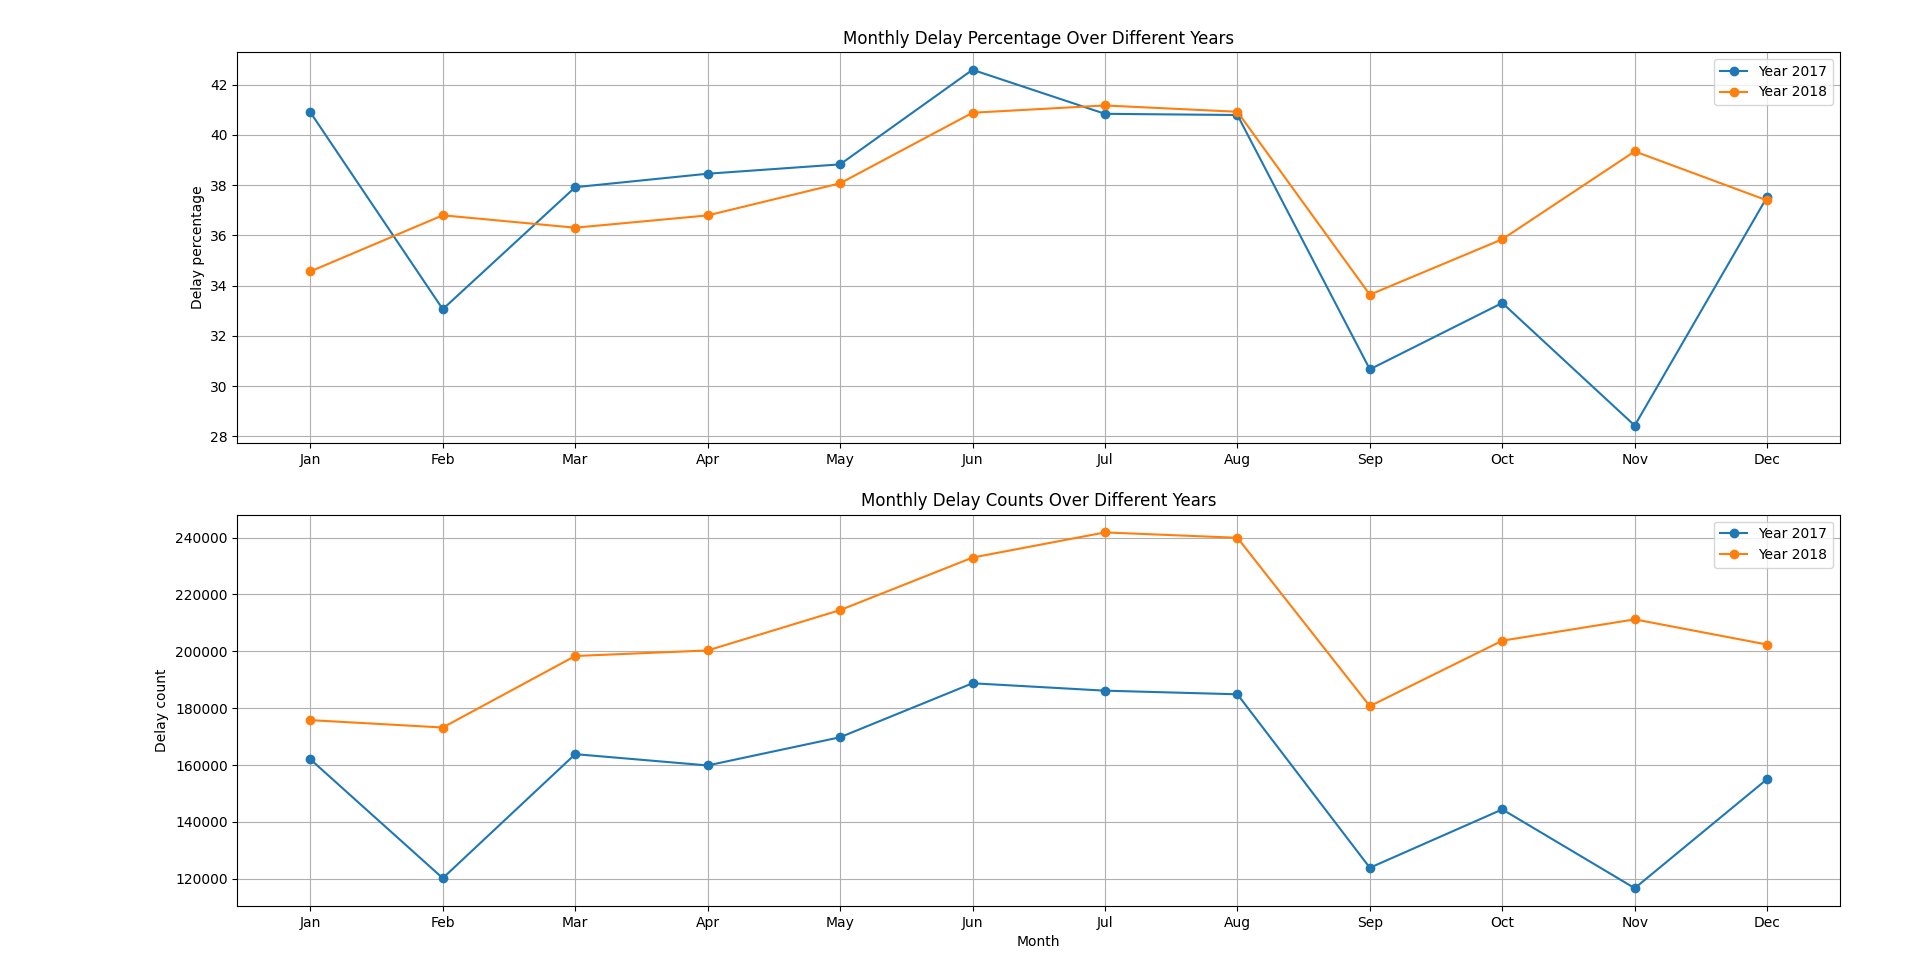
\includegraphics[scale=0.22]{plot1}
	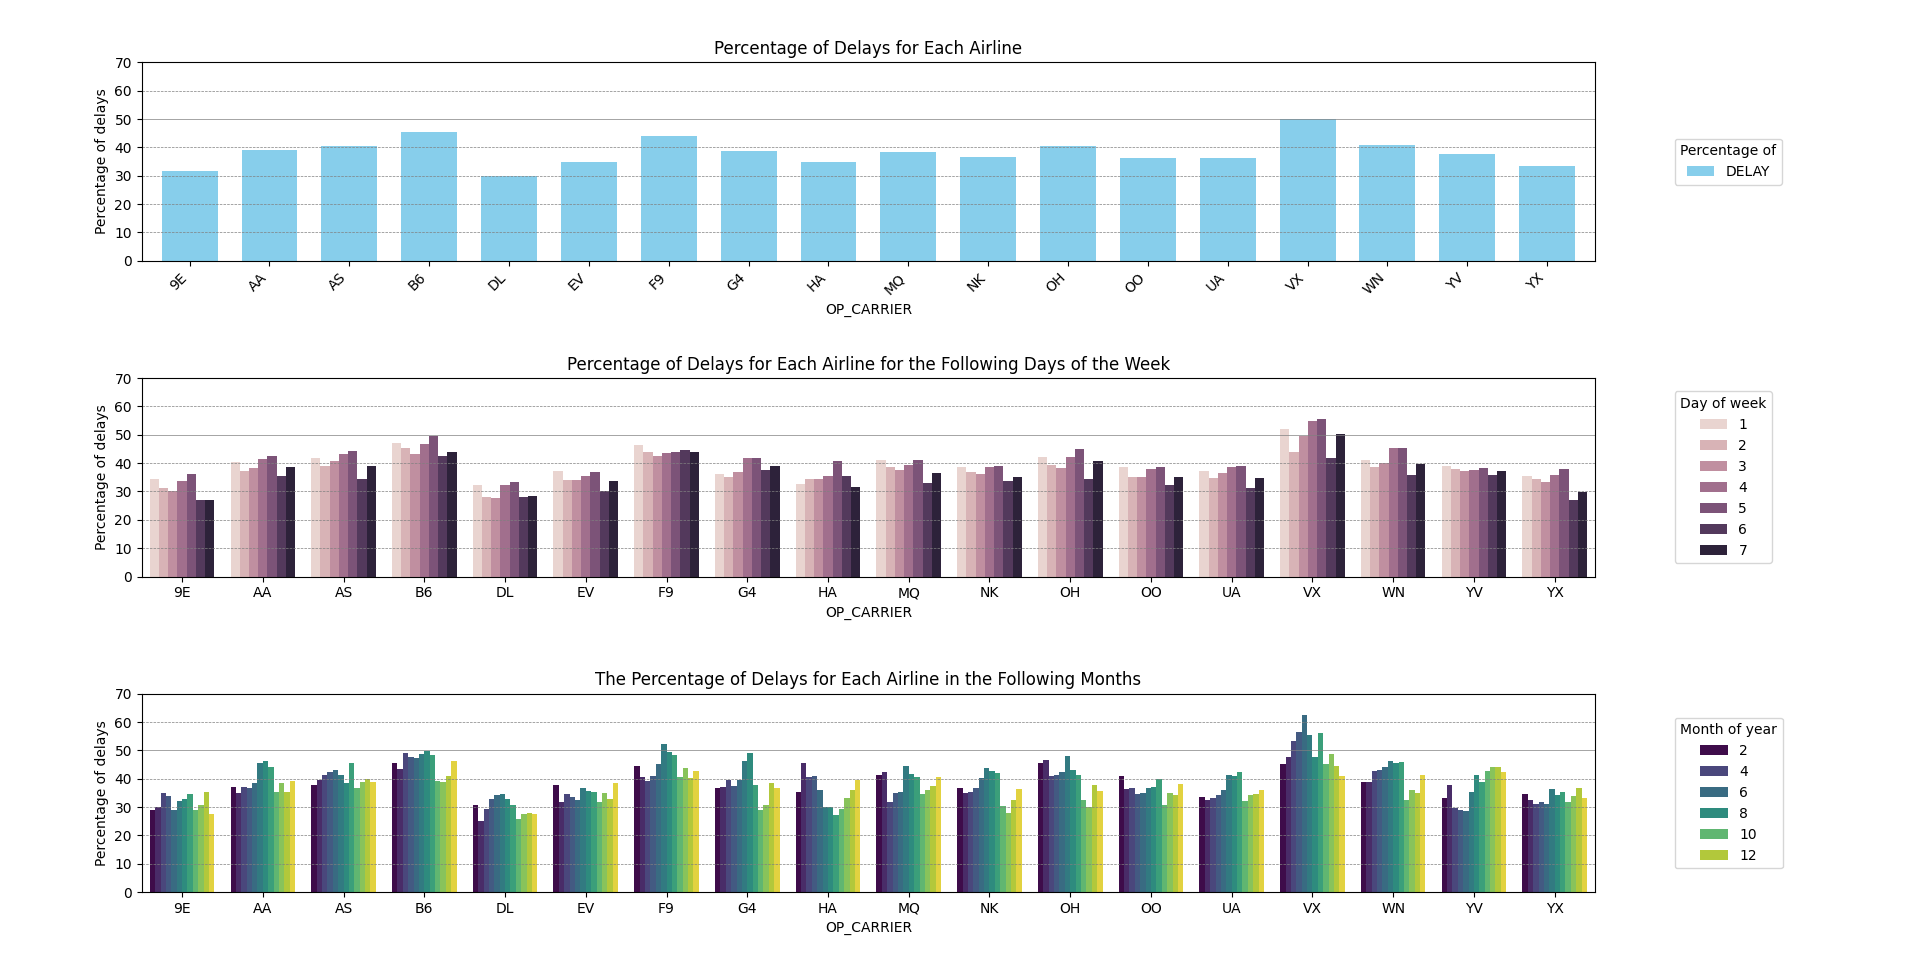
\includegraphics[scale=0.25]{plot2}
	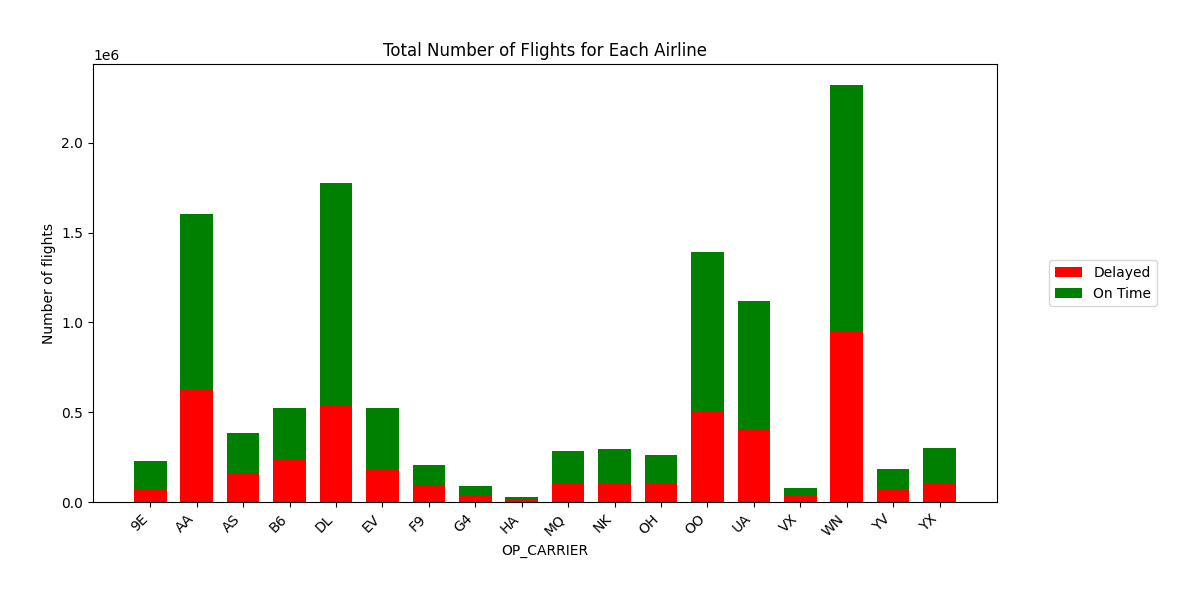
\includegraphics[scale=0.4]{plot3}
	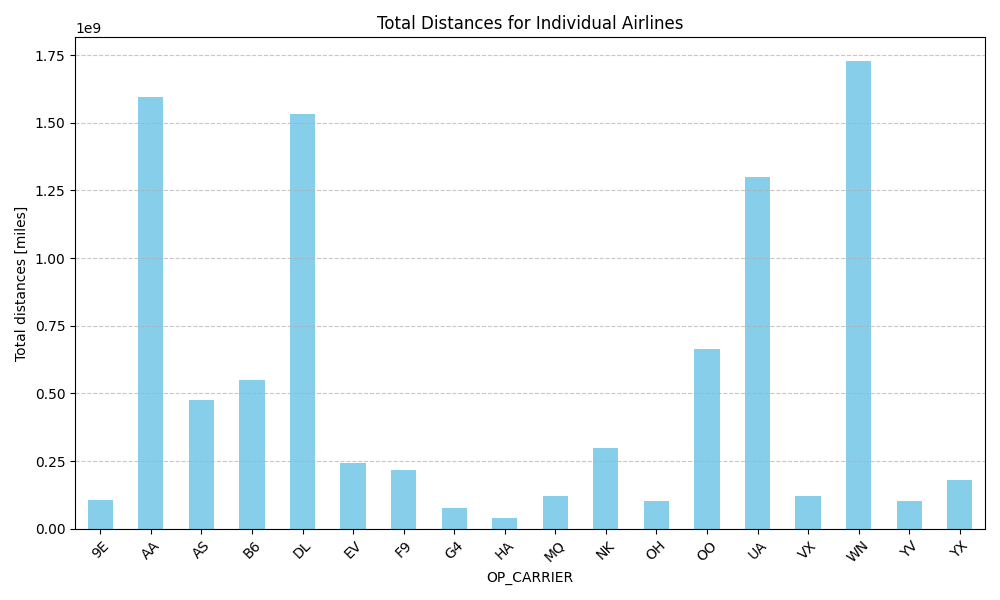
\includegraphics[scale=0.4]{plot4}	
	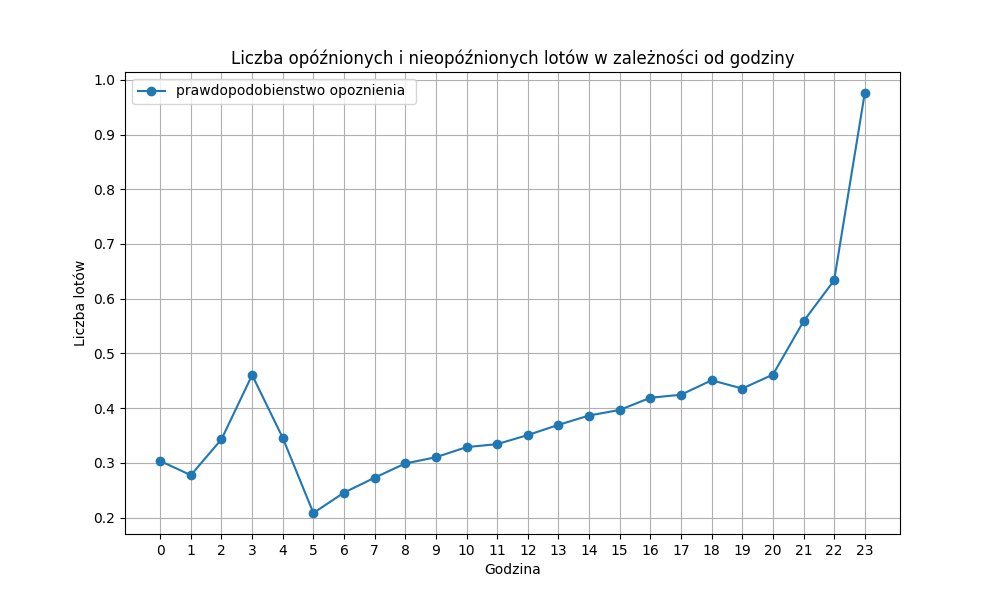
\includegraphics[scale=0.4]{delay_plot}
	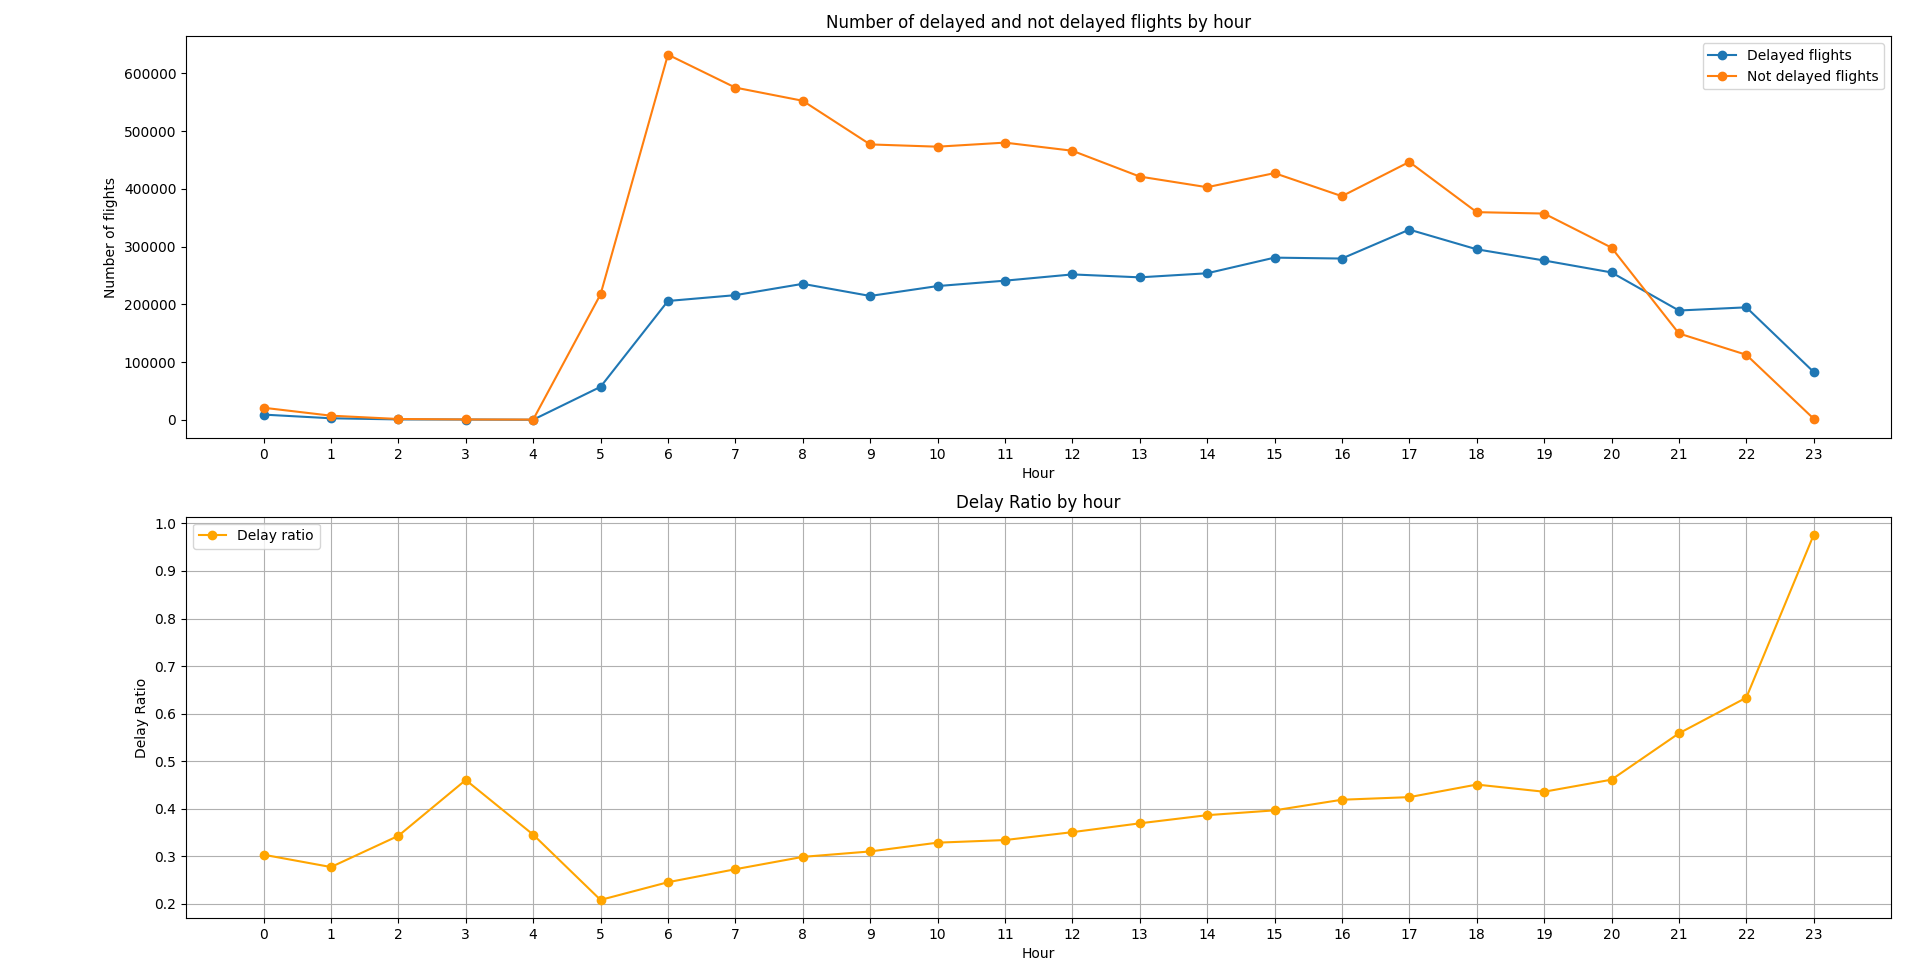
\includegraphics[scale=0.25]{delay_plot2}

\newpage

\section{Machine learning part}
In this section we will consider machine learning algorithms. All of them are sklearn library based classes.
\subsection{Decision tree}
We ran Decision Trees with gini criterion from max\_depth ranging from 4 to 20.
From our experience, the best results we achieved with depth equal to 17. We achived 66\% accuracy. It's the best accuracy we could score in our
models.

\subsection{Naive Bayes}
Our model was trained on GaussianNB() classifier. Furthermore, we used GridSearchCV() class, which helped us
to choose best var\_smoothing parameter (portion of the largest variance of all features that is added to variances for calculation stability [from
documentation]). It turned out that best accuracy was achieved with smoothing equal to $10^{-9}$ and returning 63\% of accuracy. Testing lower 
smoothing values resulted in same accuracy.

\subsection{Miscellaneous models}
	\begin{itemize}
	\item ADABoostClassifier with SAMME algorithm and 100 estimators: 57\%
	\item Random Forest Classifier with 10\_000 min\_leafs(minimum samples required to be a leaf): 64\%
	\item SGD Classifier with best alpha equal to 0.0001 and max\_iter equal to 3000 gives 62.5\% accuracy
	\end{itemize}

\subsection{4fun models}
In this section we considered models that were extremely bad or did not fall under machine learning algorithms category (neural networks).

\subsubsection{Online model}
Accuracy - around 33\%. We tried to implement using divided datasets and train model by SGD classifier (stochastic gradient descent).
It was bad.

\subsubsection{Neural network}
Accuracy - around 67\%. It was kind of good result.  I don't know what this code does. help


\section{Conclusion}
Even though we think 67\% accuracy might be too low, project taught us numerous important things. First and foremost, data exploration, that is
working with huge datasets and handling large api queries.  Then we had to process data to work with it. Problems started when we started machine learning
section. One thing that could be the cause of failure might be too much of data and lack of knowledge. Maybe we could have used time series? We
could easily see the correlation between time and delay of flights.


\end{document} 


























